The learning-in-the-quantum journey continues: after interacting in a model-free way with quantum systems of light, we will here pose the learning task differently. The agnostic drama will be diminished: we will now profit from our knowledge of quantum theory to aid the discover of novel protocols in NISQ quantum computing. Instead of treating quantum devices as black-boxes, we will inject some knowledge by introducing a semi-agnostic algorithm that discovers useful NISQ circuits. While the agent will have perfect control of the task at hand, the nature of the problem she is faced towards is so hard, that the solutions are unknown to us. Thus, the agent learns in the twilight: while knowledge of NISQ quantum-computing is available, the nature of the solutions she is seeking for is completely unknown.

Here, we will focus on how currently available quantum computers can be used for a wide range of problems, ranging from ground-state preparation and training quantum autoencoders to compiling unitary transformations on native hardware. As discussed in Sec.~\ref{sec:1_nisq}, it seems natural to adjust the learning algorithm to the task at hand, but doing it is often hard because the learning scenarios are far from ideal.

While in the introductory Section we have stressed these difficulties for the NISQ scenario, let us remark that big efforts have been carried out by the machine-learning community in the recent years in order to injecting prior knowledge into deep-learning architectures~\cite{9363511, ShlezingerNir2020VADL}. Overall, the design of a machine-learning algorithm, when taking into account the structure that a potential solution shall obey, is subtle and (as expected) problem-dependent. An example of this is given by Convolutional Neural Networks~\cite{CNN,CNN1,CNN2}, designed in such a way to sequentially process an image in a task-oriented manner. Here, the network is able to identify \textit{features} that are invariant under translation-like transformations, such as eyes or mouths in human pictures, and thus exploits the correlations hidden in the image. %As expected, these architectures are specifically-tailored for pattern recognition in images, and thus their performance on different tasks is generally poor.

However, by such prior-knowledge injection we unavoidable induce some bias to model, and we can readily elucidate a tradeoff. In this Chapter, rather than specifically-tailoring an algorithm to come up with a task-oriented solution, we will study the performance of a general-purposed algorithm, which adapts its structure to the specific cost-function at hand, by means of machine-learning inspired techiques.

We will focus on NISQ computing, which were previously discussed in Sec.~\ref{sec:1_nisq}. Here, an intermediate-scale (of about $\sim$100 qubits) noisy quantum device needs to be configured as a special-purpose machine. A promising route to do so is given by Variational Quantum Algorithms (VQAs), as discussed in Sec.~\ref{ssec:1_nisq_vqa}. In VQAs, a parametrized quantum circuit (PQC) is used to estimate cost-function values, whose minima encodes solutions to the problem at hand. In order to reach such minima, a classical algorithm is used to optimize available degrees of freedom such as qubit-rotation values, or even circuit's structure. The latter plays a crucial role in NISQ computing: while the presence of noise essentially fordibs the implementation of large-depth circuits, special care must be taken even when dealing with shallow circuits due to the appearence of Barren Plateaus (BPs). As discussed in Sec.~\ref{ssec:1_nisq_barrenplateaus}, under the pressence of a BP, estimating cost-minimizing directions is very hard, since the gradients exponentially concentrate around zero, which in turn implies that any optimizer will effectively get stucked. Addressing the BP issue currently constitutes one of the major research directions in the field of NISQ computing. Here, the ansatz used for the quantum circuit (\textit{e.g.} the structure under which quantum gates act on the available qubits) plays a fundamental role, and developing tools to discover useful quantum-circuit structures that can be trained under the VQA framework is of utmost importance.

\begin{figure}[h!]
\centering
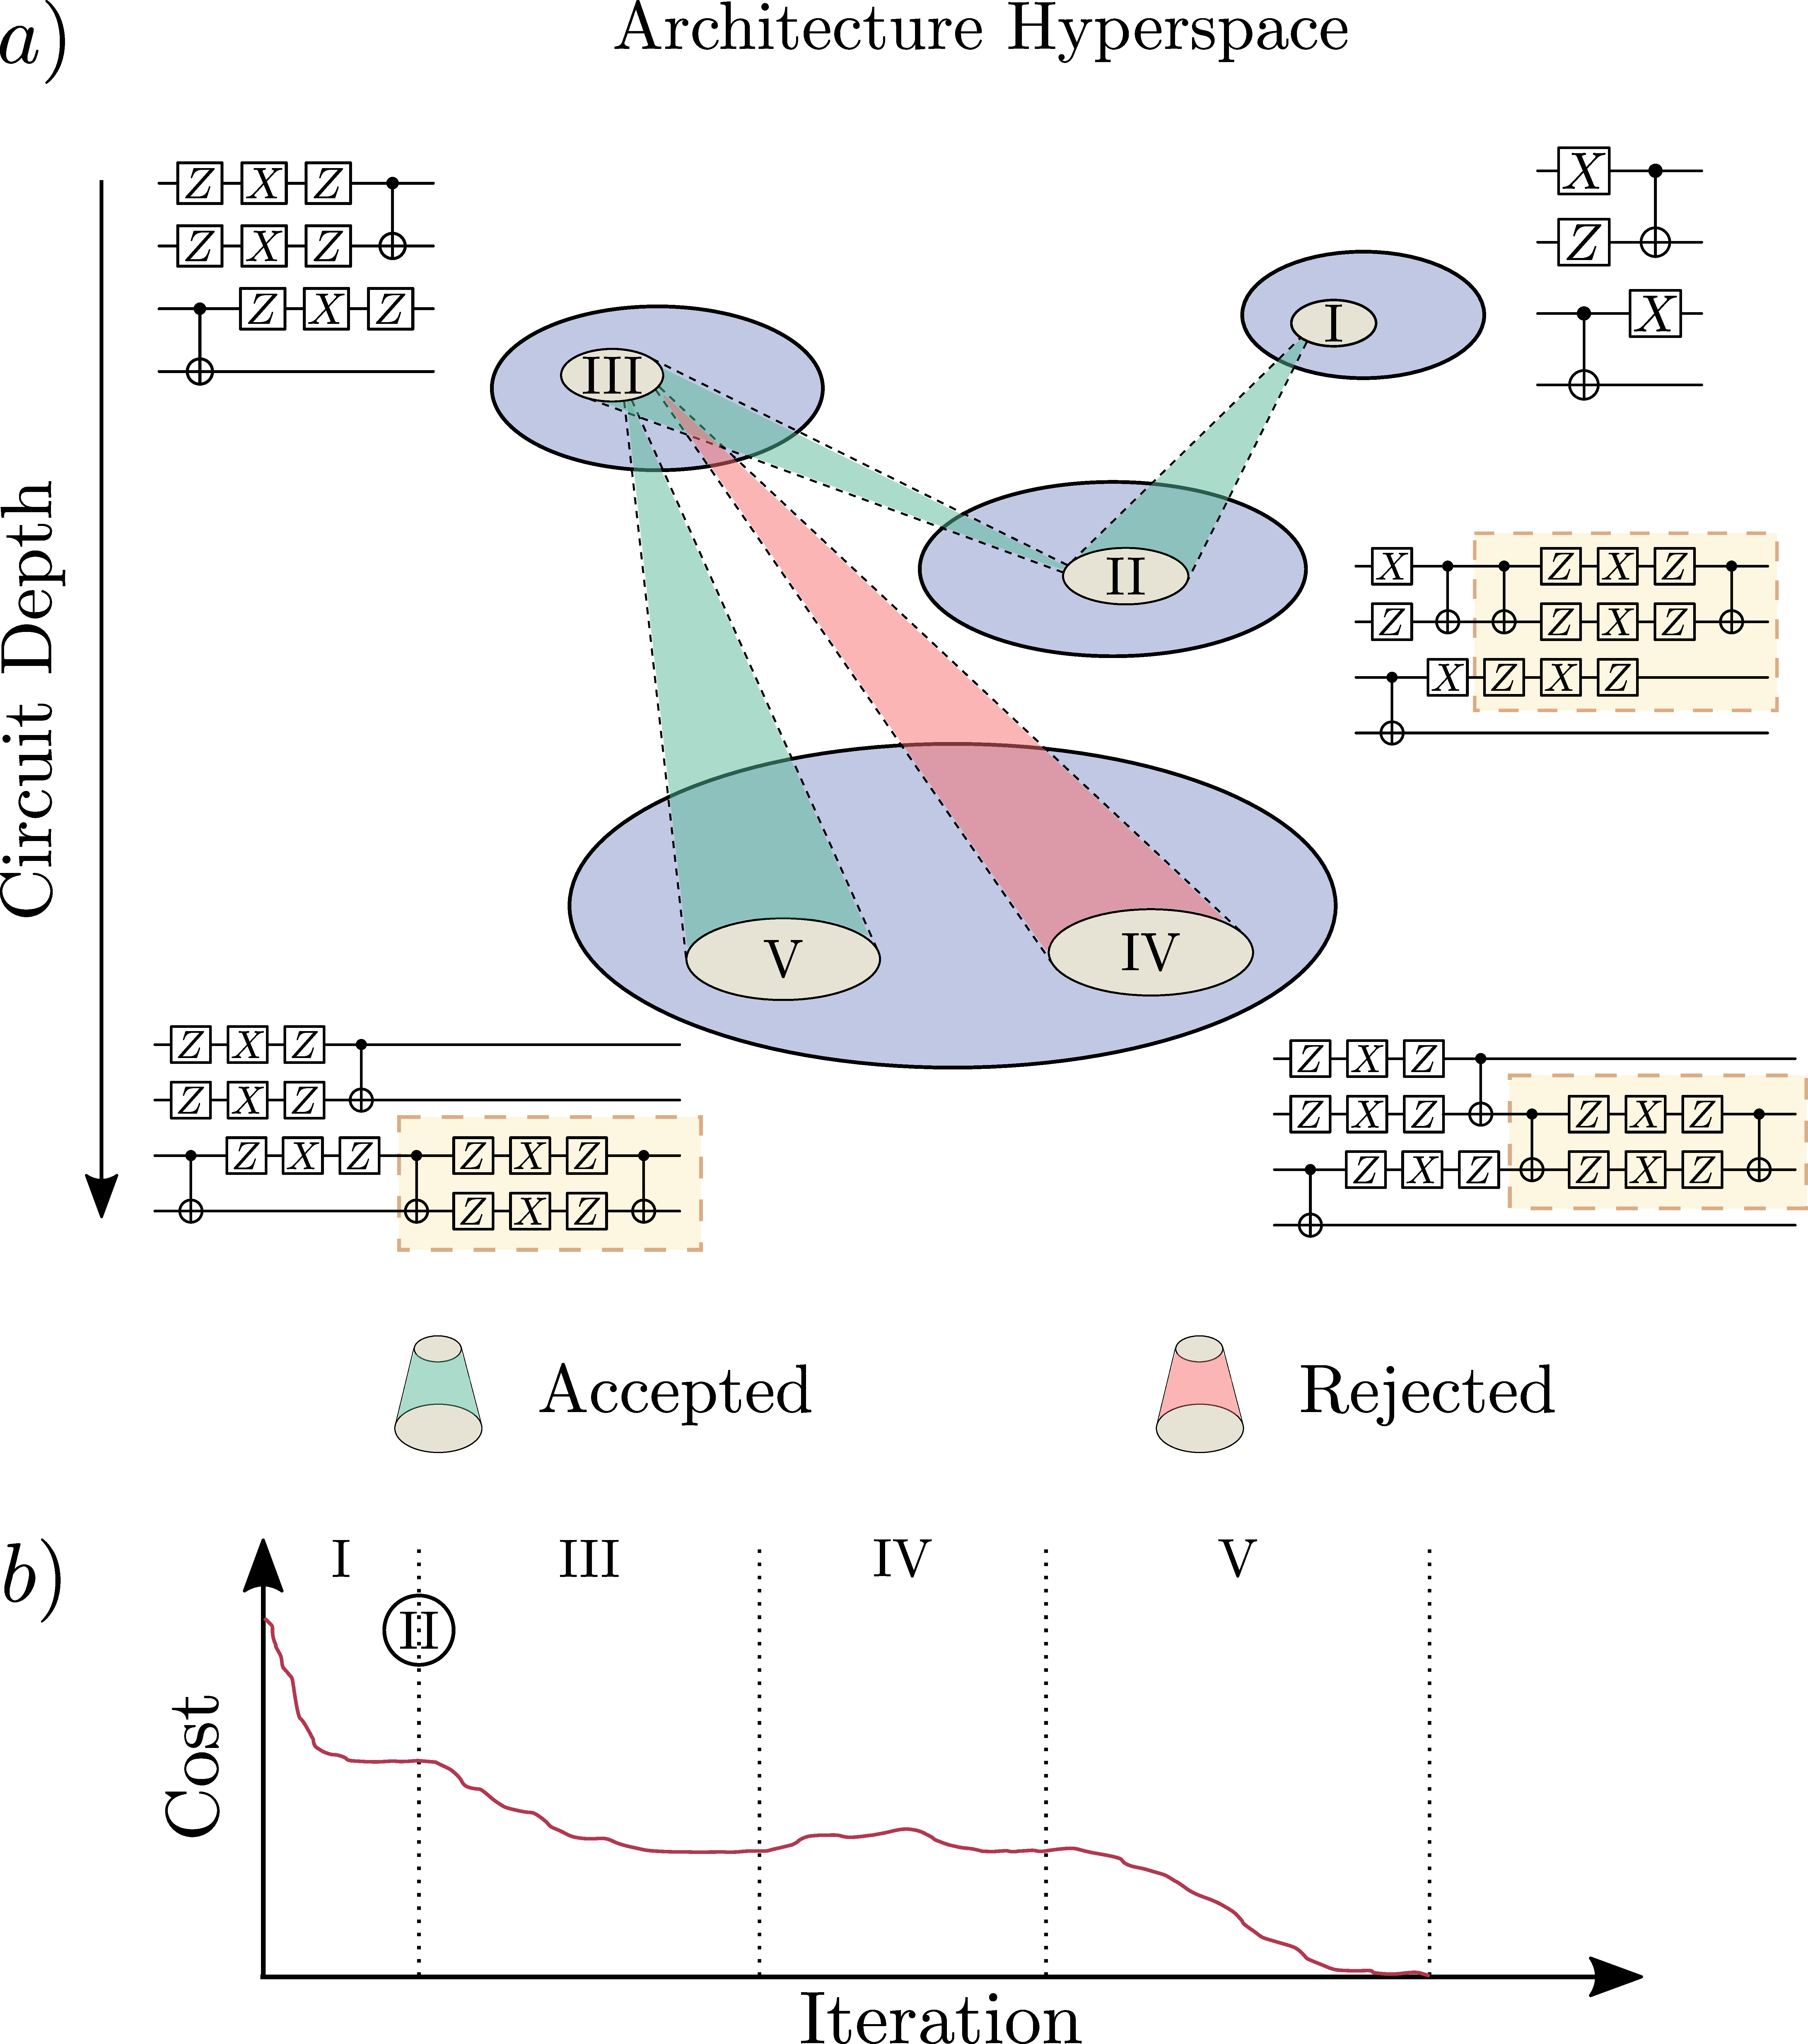
\includegraphics[width=.8\textwidth]{Figures/VANS/Fig1.pdf}
\caption{{\small We show a schematic diagram of the VAns algorithm. \textit{(a)} VAns explores the hyperspace of architectures of parametrized quantum circuits to create short depth ansatzes for VQA applications. VAns takes a (potentially non-trivial) initial circuit (step I) and optimizes its continuous parameters $\thv$ until convergence. At each step, VAns inserts blocks of gates into the circuit which are initialized to the identity (indicated in a box in the figure), so that the ansatzes at contiguous steps belong to an equivalence class of circuits leading to the same cost value (step II). VAns then employs a classical algorithm to simplify the circuit by eliminating gates and finding the shortest circuit (step II to III). The ovals represent subspaces of the architecture hyperspace connected through VAns. While some regions may be smoothly connected by placing identity resolutions, VAns can also explore regions that are not smoothly connected via a gate-simplification process. VAns can either reject (step IV) or accept (step V) modifications in the circuit structure. Here $Z$ ($X$) indicates a rotation about the $z$ ($x$) axis. \textit{(b)} Schematic representation of the cost function value versus the number of iterations for a typical VAns implementation which follows the steps in \textit{(a)}.}}
\label{fig:schematic}
\end{figure}

\afterpage{\clearpage}

To this end, we combine several features of recently proposed methods and introduce the Variable Ansatz (VAns) algorithm~\cite{bilkis2021semi} to generate variable structure ansatzes for generic VQA applications. As shown in Fig.~\ref{fig:schematic}, VAns iteratively grows the parameterized quantum circuit by adding blocks of gates initialized to the identity, but also prevents the circuit from over-growing by removing gates and compressing the circuit at each iteration. In this sense, VAns produces shallow circuits that are more resilient to noise, and that have less trainable parameters to avoid trainability issues. Our approach provides a simple yet effective way to address the ansatz design problem, without resorting to resource-expensive computations similar to recently evolutionary-oriented proposals.

Our algorithm is inspired by the strong presence of noise in NISQ devices. As such, it potentially hinders any successful application of NISQ computers. In this context, we should take advantage of every component of the quantum device that could be optimized over, and this generally includes the circuit's layout. In this regard, some approaches ---as EVQE~\cite{rattew2019domain} or MoG-VQE~\cite{chivilikhin2020mog} ---have been introdued in the past, as discussed in Sec.~\ref{ssec:1_nisq_vans_bp}. VAns algorithm differs from them in at least two important aspects: \textit{(i)} it considers general cost functions, and thus can be considered a general-purposed quantum-machine learning algorithm, and \textit{(ii)} the method incorporates knowledge on quantum computing via specific circuit compression rules.

Thus, the learning problem we are dealing with consists in finding cost-minimizing quantum circuits, where not only the parameters can be optimized, but also the structure of the circuit itself. While some light is shed into the learning problem through the aforementioned compression rules, an important \textit{learning-in-the-darkness} component remains. In particular, no structure is imposed on how our algorithm grows the quantum circuit, and at each time-step quantum gates are randomly placed across the circuit, acting on qubits that are also randomly selected. Thus, the learning paradigm departs from the one considered in Chapter~\ref{chapter:RLCOH}, and rather than assuming complete ignorance of the setting, the agent (VAns algorithm) is now equipped with partial information about the setting, henceforth it learns in the twilight through the VAns algorithm, which we now turn to explain in detail.
